\documentclass[tikz, border=5mm]{standalone}
\usepackage{tikz}
\usetikzlibrary{positioning, arrows.meta, calc}

\begin{document}
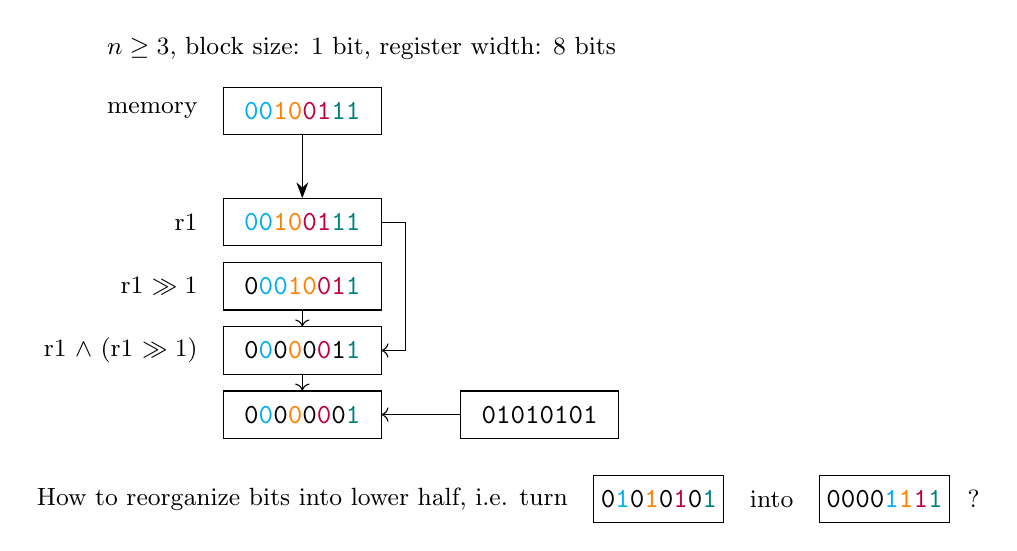
\begin{tikzpicture}[
    node distance=2mm and 5mm, % vertical and horizontal node distance
    bitbox/.style={draw, font=\ttfamily, inner sep=2.5pt, minimum height=6mm, minimum width=20mm}, % Adjusted min width for 8 bits
    labelstyle/.style={font=\small},
    operationstyle/.style={font=\Large\ttfamily} % Style for the & symbol
]

% Header text
\node (ex_label) [labelstyle] {\(n\geq 3\), block size: 1 bit, register width: 8 bits};

% Memory line
\node (mem_label) [labelstyle, below=8mm of ex_label.west, anchor=west] {memory};
\node (mem_val) [bitbox, right=2mm of mem_label] {{\color{cyan}00}{\color{orange}10}{\color{purple}01}{\color{teal}11}};

% r1
\node (r1_val) [bitbox, below=8mm of mem_val] {{\color{cyan}00}{\color{orange}10}{\color{purple}01}{\color{teal}11}};
\node (r1_label) [labelstyle, left=2mm of r1_val] {r1};
\draw[-{Stealth[length=2mm, width=1.5mm]}] (mem_val.south) -- (r1_val.north);

% r1 >> 1
\node (r1_shifted_val) [bitbox, below=of r1_val] {0{\color{cyan}00}{\color{orange}10}{\color{purple}01}{\color{teal}1}};
\node (r1_shifted_label) [labelstyle, left=2mm of r1_shifted_val] {r1 $\gg 1$};

% AND Mask
\node (and_mask_val) [bitbox, below=of r1_shifted_val] {0{\color{cyan}0}0{\color{orange}0}0{\color{purple}0}1{\color{teal}1}};
\node (and_mask_label) [labelstyle, left=2mm of and_mask_val] {r1 $\land$ (r1 $\gg 1$)};

% Result of AND
\node (and_result_val) [bitbox, below=of and_mask_val] {0{\color{cyan}0}0{\color{orange}0}0{\color{purple}0}0{\color{teal}1}};

\node (final_mask_val) [bitbox, right=10mm of and_result_val] {01010101};
\draw[->] (final_mask_val) -- (and_result_val);
\draw[->] (and_mask_val) -- (and_result_val);

% Connecting lines and & symbol for the AND operation
% Create a coordinate for the vertical line segment
\coordinate (and_line_top) at ($(r1_val.east)+(3mm,0)$);
\coordinate (and_line_bottom) at ($(and_mask_val.east)+(3mm,0)$);
\draw (r1_val.east) -- (and_line_top);
\draw[<-] (and_mask_val.east) -- (and_line_bottom);
\draw (and_line_top) -- (and_line_bottom); % Vertical line
\draw[->] (r1_shifted_val.south) -- (and_mask_val);

% Arrow from the & symbol (or the space it occupies) to the result
% We'll draw it from a point to the right of the vertical line
\coordinate (and_op_midpoint) at ($(and_line_top)!0.5!(and_line_bottom)$);

\node (q2_text1) [labelstyle, below=5mm of and_result_val, anchor=north] {How to reorganize bits into lower half, i.e. turn};
\node (q2_box1) [bitbox, right=2mm of q2_text1, minimum width=15mm] {0{\color{cyan}1}0{\color{orange}1}0{\color{purple}1}0{\color{teal}1}};
\node (q2_text_into) [labelstyle, right=2mm of q2_box1] {into};
\node (q2_box2) [bitbox, right=2mm of q2_text_into, minimum width=15mm] {0000{\color{cyan}1}{\color{orange}1}{\color{purple}1}{\color{teal}1}};
\node (q2_qmark) [labelstyle, right=1mm of q2_box2] {?};


\end{tikzpicture}
\end{document}
